\subsubsection{Analisi al variare di T}
Per quanto riguarda le prestazioni al variare del valore del timeout,
si osserva (figura \ref{t}) che vi è una crescita lineare del tempo impiegato all'aumentare del
parametro T nel caso di timeout fisso.\\
Nel caso di timeout adattativo, per perdite poco o mediamente frequenti,
il tempo impiegato converge ad un valore costante
proporzionale alla probabilità di perdita,
mentre si conferma molto variabile in caso di elevata probabilità di perdita. 
\begin{figure}[!hp]
	\centering
	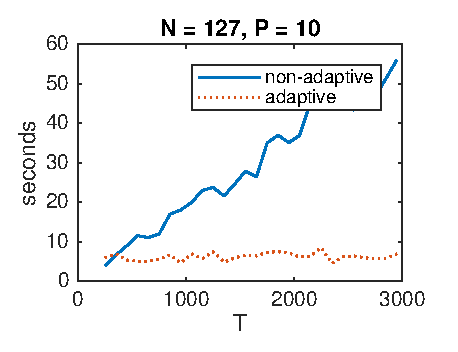
\includegraphics[scale=0.8]{images/T_N127_P10}
	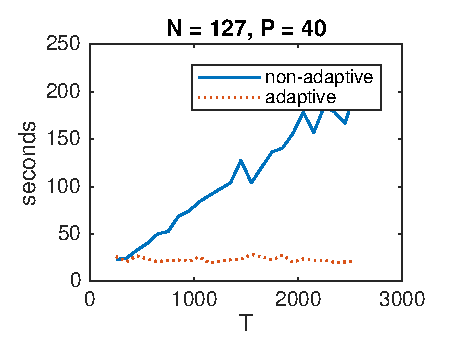
\includegraphics[scale=0.8]{images/T_N127_P40}
	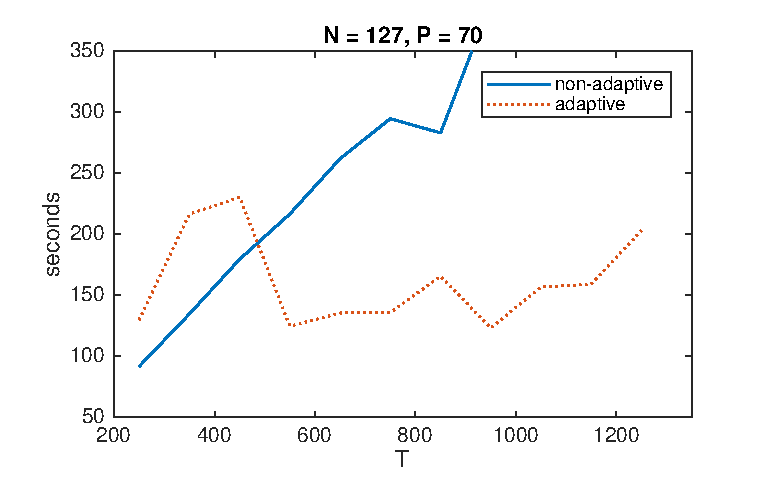
\includegraphics[scale=0.8]{images/T_N127_P70}
	\caption{prestazioni al variare del valore del timeout T,
			 ampiezza finestra N = 127, probabilità di perdita bassa (P = 10\%),
			 media (P = 40\%) e alta (P = 70\%)}
	\label{t}
\end{figure}
